\begin{flushright} {\tiny {\color{gray} (tikz\_needicon.tex)}} \end{flushright}
%~~~~~~~~~~~~~~~~~~~~~~~~~~~~~~~~~~~~~~~~~~~~~~~~~~~~~~~~~~~~~~~~~~~~~~~~~~~~~~~~~~~~~~~~~~~~~~~~~~


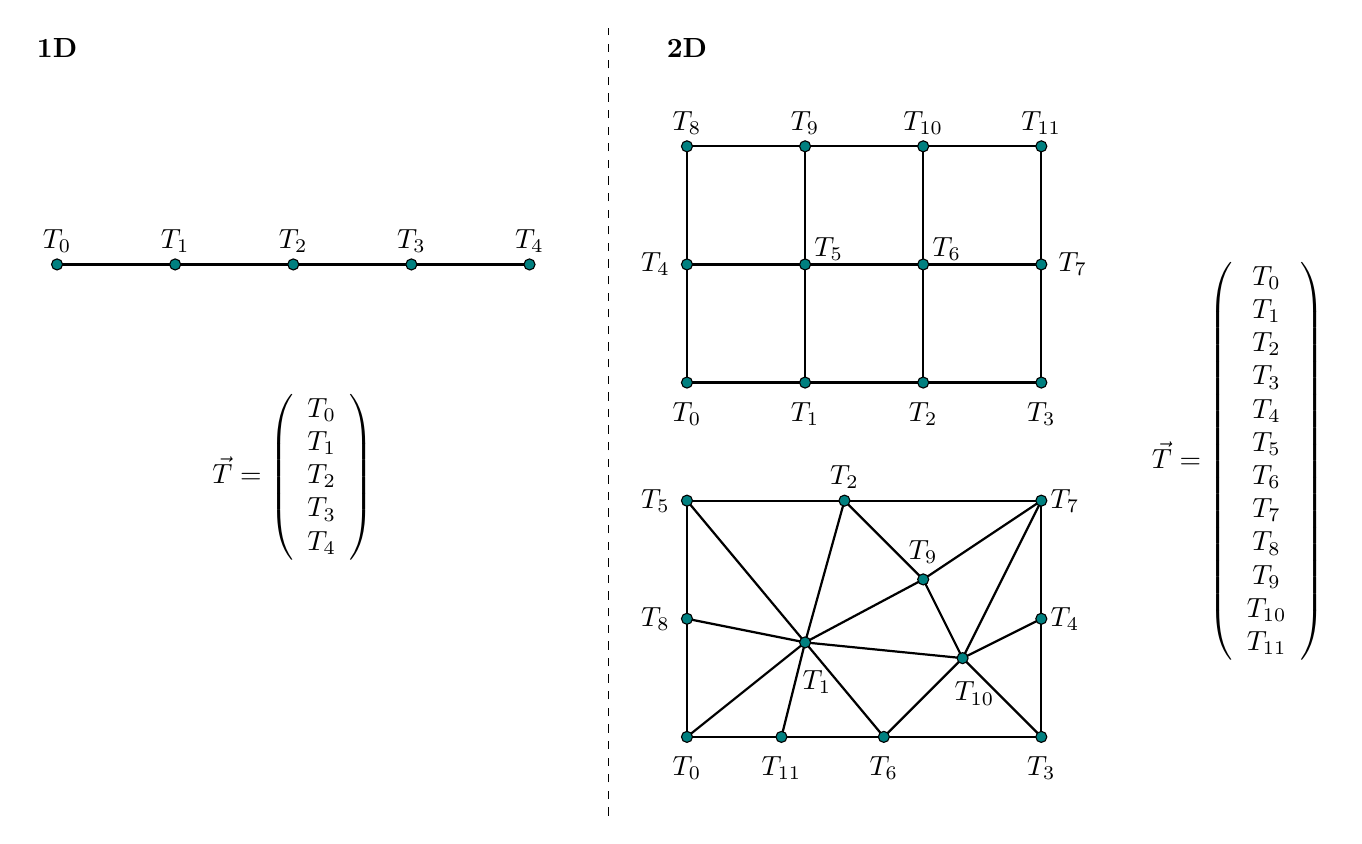
\begin{tikzpicture}
%\draw[step=0.5cm,gray,very thin] (0,0) grid (17,10); 

\node[] at (1,9.75) {\bf 1D};

\draw[thick] (1,7)--(7,7);
\draw[black,fill=teal] (1,7) circle (2pt);
\draw[black,fill=teal] (2.5,7) circle (2pt);
\draw[black,fill=teal] (4,7) circle (2pt);
\draw[black,fill=teal] (5.5,7) circle (2pt);
\draw[black,fill=teal] (7,7) circle (2pt);

\node[] at (1,7.3) {$T_0$};
\node[] at (2.5,7.3) {$T_1$};
\node[] at (4,7.3) {$T_2$};
\node[] at (5.5,7.3) {$T_3$};
\node[] at (7,7.3) {$T_4$};

\node[] at (4,4.3) {
$\vec{T}=\left(
\begin{array}{c}
T_0 \\ T_1 \\ T_2 \\ T_3 \\ T_4
\end{array}
\right)$};

%%%%%%%%%%%%%%%%%%%%%%%%%%%%%%%%%%%%%%%%%55
\draw[dashed] (8,0)--(8,10); 

\node[] at (9,9.75) {\bf 2D};

\draw[thick](9,5.5) rectangle (13.5,8.5);
\draw[thick](9,7)--(13.5,7);
\draw[thick](10.5,5.5)--(10.5,8.5);
\draw[thick](12,5.5)--(12,8.5);

\node[] at (16,4.5) {
$\vec{T}=\left(
\begin{array}{c}
T_0 \\ T_1 \\ T_2 \\ T_3 \\ T_4 \\
T_5 \\ T_6 \\ T_7 \\ T_8 \\ T_9 \\ T_{10} \\ T_{11}
\end{array}
\right)$};

\draw[black,fill=teal] (9,5.5) circle (2pt);
\draw[black,fill=teal] (10.5,5.5) circle (2pt);
\draw[black,fill=teal] (12,5.5) circle (2pt);
\draw[black,fill=teal] (13.5,5.5) circle (2pt);

\draw[black,fill=teal] (9,7) circle (2pt);
\draw[black,fill=teal] (10.5,7) circle (2pt);
\draw[black,fill=teal] (12,7) circle (2pt);
\draw[black,fill=teal] (13.5,7) circle (2pt);

\draw[black,fill=teal] (9,8.5) circle (2pt);
\draw[black,fill=teal] (10.5,8.5) circle (2pt);
\draw[black,fill=teal] (12,8.5) circle (2pt);
\draw[black,fill=teal] (13.5,8.5) circle (2pt);

\node[] at (9,5.1) {$T_0$};
\node[] at (10.5,5.1) {$T_1$};
\node[] at (12,5.1) {$T_2$};
\node[] at (13.5,5.1) {$T_3$};
\node[] at (8.6,7) {$T_4$};

\node[] at (10.8,7.2) {$T_5$};
\node[] at (12.3,7.2) {$T_6$};

\node[] at (13.9,7) {$T_7$};

\node[] at (9,8.8) {$T_8$};
\node[] at (10.5,8.8) {$T_9$};
\node[] at (12,8.8) {$T_{10}$};
\node[] at (13.5,8.8) {$T_{11}$};

%%%%%%%%%%%%%%%%%%%%%%%%%%%%%%%%%%%%%%%5
%triangular mesh

\draw[thick](9,1) rectangle (13.5,4);


\draw[thick](9,1)--(10.5,2.2)--(12,3)--(13.5,4);
\draw[thick](9,4)--(10.5,2.2)--(12.5,2)--(13.5,1);
\draw[thick](11,4)--(12,3)--(12.5,2)--(13.5,2.5);
\draw[thick](13.5,4)--(12.5,2)--(11.5,1)--(10.5,2.2)--(9,2.5);
\draw[thick](10.2,1)--(10.5,2.2)--(11,4);


\draw[black,fill=teal] (9,1) circle (2pt);
\draw[black,fill=teal] (10.2,1) circle (2pt);
\draw[black,fill=teal] (11.5,1) circle (2pt);
\draw[black,fill=teal] (13.5,1) circle (2pt);

\draw[black,fill=teal] (9,2.5) circle (2pt);
\draw[black,fill=teal] (10.5,2.2) circle (2pt);
\draw[black,fill=teal] (12,3) circle (2pt);
\draw[black,fill=teal] (12.5,2) circle (2pt);
\draw[black,fill=teal] (13.5,2.5) circle (2pt);

\draw[black,fill=teal] (9,4) circle (2pt);
\draw[black,fill=teal] (11,4) circle (2pt);
\draw[black,fill=teal] (13.5,4) circle (2pt);

\node[] at (9,0.6) {$T_0$};
\node[] at (10.2,0.6) {$T_{11}$};
\node[] at (11.5,0.6) {$T_6$};
\node[] at (13.5,0.6) {$T_3$};

\node[] at (8.6,2.5) {$T_8$};
\node[] at (8.6,4) {$T_5$};
\node[] at (11,4.3) {$T_2$};
\node[] at (13.8,4) {$T_7$};
\node[] at (13.8,2.5) {$T_4$};

\node[] at (12,3.35) {$T_9$};
\node[] at (12.65,1.55) {$T_{10}$};

\node[] at (10.65,1.7) {$T_1$};

\end{tikzpicture}
